\documentclass[border=8pt]{standalone}
\usepackage[T1]{fontenc}\usepackage[utf8]{inputenc}
\usepackage{helvet}\renewcommand{\familydefault}{\sfdefault}
\usepackage{tikz,xcolor}
\usetikzlibrary{arrows.meta,positioning,shapes.geometric,shapes.multipart,calc,fit,backgrounds,decorations.markings}
\definecolor{ink}{HTML}{1E1B16}\definecolor{paper}{HTML}{FBF8F2}\definecolor{clay}{HTML}{B5482A}\definecolor{soft}{HTML}{F1E9DA}\definecolor{pine}{HTML}{24402F}
\tikzset{
  every node/.style={font=\small,text=ink},
  >=Stealth, line/.style={draw=ink,line width=0.8pt},
  cls/.style={rectangle split,rectangle split parts=3,draw=ink,line width=0.8pt,fill=soft,align=left,inner xsep=6pt,inner ysep=4pt,
              rectangle split part align={center,left,left},minimum width=3.0cm},
  cls2/.style={rectangle split,rectangle split parts=2,draw=ink,line width=0.8pt,fill=soft,align=left,inner xsep=6pt,inner ysep=4pt,
              rectangle split part align={center,left},minimum width=3.0cm},
  box/.style={rectangle,draw=ink,line width=0.8pt,fill=soft,align=center,inner sep=5pt,minimum height=0.8cm},
  state/.style={rectangle,rounded corners=8pt,draw=ink,line width=0.8pt,fill=soft,align=center,inner sep=6pt,minimum width=2.2cm,minimum height=0.9cm},
  act/.style={rectangle,rounded corners=10pt,draw=ink,line width=0.8pt,fill=soft,align=center,inner sep=5pt,minimum width=2.4cm,minimum height=0.8cm},
  dec/.style={diamond,draw=ink,line width=0.8pt,fill=soft,inner sep=1pt,minimum width=0.9cm,minimum height=0.9cm},
  uc/.style={ellipse,draw=ink,line width=0.8pt,fill=soft,align=center,inner sep=3pt,minimum width=3.2cm,minimum height=1.0cm},
  note/.style={rectangle,draw=ink,line width=0.6pt,fill=yellow!12,align=left,inner sep=4pt,font=\footnotesize},
  lab/.style={font=\footnotesize,fill=paper,inner sep=1.5pt},
  err/.style={},
}
\newcommand{\actor}[3]{% x,y,label
  \draw[line width=0.8pt] (#1,#2+0.55) circle (0.17);
  \draw[line width=0.8pt] (#1,#2+0.38)--(#1,#2-0.15) (#1-0.3,#2+0.22)--(#1+0.3,#2+0.22) (#1,#2-0.15)--(#1-0.25,#2-0.6) (#1,#2-0.15)--(#1+0.25,#2-0.6);
  \node[font=\small] at (#1,#2-0.9) {#3};}
\begin{document}
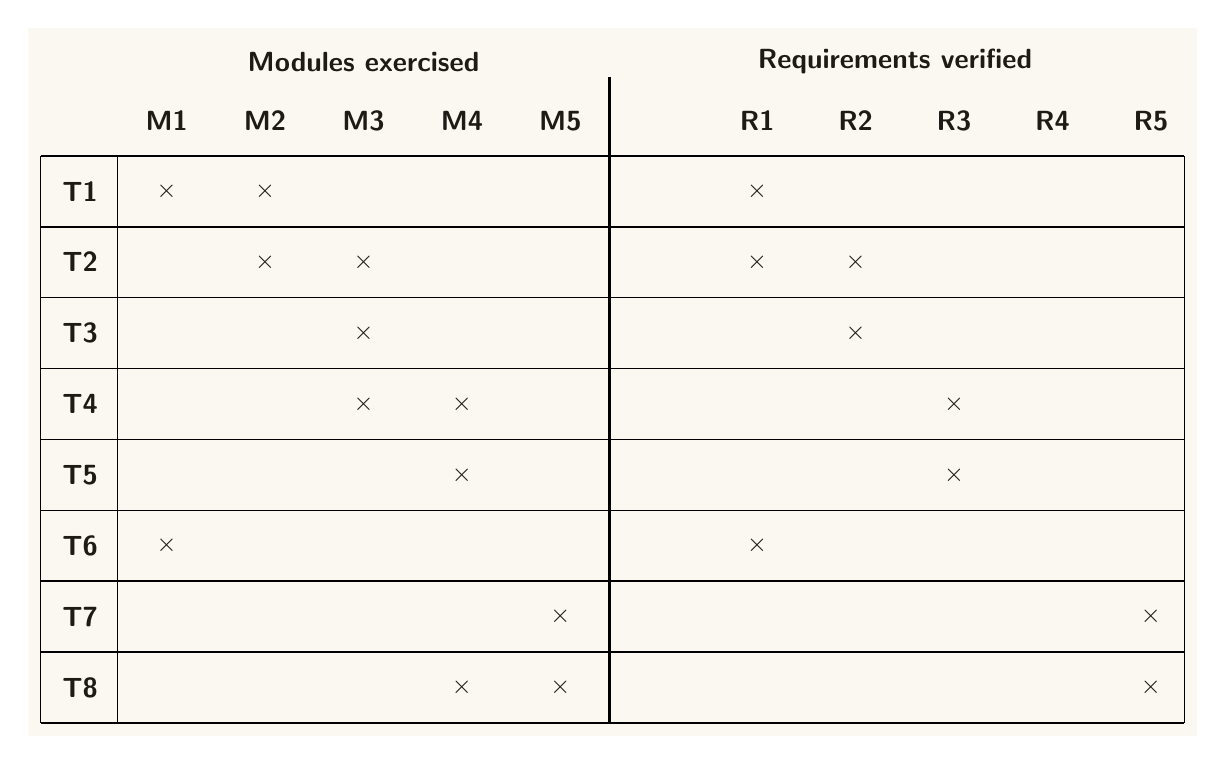
\begin{tikzpicture}[background rectangle/.style={fill=paper},show background rectangle]
\node[font=\bfseries] at (3.900000,1.2) {Modules exercised};\node[font=\bfseries] at (10.650000,1.2) {Requirements verified};\node[font=\bfseries] at (1.4,0.45) {M1};
\node[font=\bfseries] at (2.65,0.45) {M2};
\node[font=\bfseries] at (3.9,0.45) {M3};
\node[font=\bfseries] at (5.15,0.45) {M4};
\node[font=\bfseries] at (6.4,0.45) {M5};
\node[font=\bfseries] at (8.9,0.45) {R1};
\node[font=\bfseries] at (10.15,0.45) {R2};
\node[font=\bfseries] at (11.4,0.45) {R3};
\node[font=\bfseries] at (12.65,0.45) {R4};
\node[font=\bfseries] at (13.9,0.45) {R5};
\node[font=\bfseries] at (0.3,-0.45) {T1};
\node at (1.4,-0.45) {$\times$};
\node at (2.65,-0.45) {$\times$};
\node at (8.9,-0.45) {$\times$};
\node[font=\bfseries] at (0.3,-1.35) {T2};
\node at (2.65,-1.35) {$\times$};
\node at (3.9,-1.35) {$\times$};
\node at (8.9,-1.35) {$\times$};
\node at (10.15,-1.35) {$\times$};
\node[font=\bfseries] at (0.3,-2.25) {T3};
\node at (3.9,-2.25) {$\times$};
\node at (10.15,-2.25) {$\times$};
\node[font=\bfseries] at (0.3,-3.1500000000000004) {T4};
\node at (3.9,-3.1500000000000004) {$\times$};
\node at (5.15,-3.1500000000000004) {$\times$};
\node at (11.4,-3.1500000000000004) {$\times$};
\node[font=\bfseries] at (0.3,-4.05) {T5};
\node at (5.15,-4.05) {$\times$};
\node at (11.4,-4.05) {$\times$};
\node[font=\bfseries] at (0.3,-4.95) {T6};
\node at (1.4,-4.95) {$\times$};
\node at (8.9,-4.95) {$\times$};
\node[font=\bfseries] at (0.3,-5.8500000000000005) {T7};
\node at (6.4,-5.8500000000000005) {$\times$};
\node at (13.9,-5.8500000000000005) {$\times$};
\node[font=\bfseries] at (0.3,-6.75) {T8};
\node at (5.15,-6.75) {$\times$};
\node at (6.4,-6.75) {$\times$};
\node at (13.9,-6.75) {$\times$};
\draw[line width=0.5pt] (-0.2,0.0) -- (14.325000000000001,0.0);
\draw[line width=0.5pt] (-0.2,-0.9) -- (14.325000000000001,-0.9);
\draw[line width=0.5pt] (-0.2,-1.8) -- (14.325000000000001,-1.8);
\draw[line width=0.5pt] (-0.2,-2.7) -- (14.325000000000001,-2.7);
\draw[line width=0.5pt] (-0.2,-3.6) -- (14.325000000000001,-3.6);
\draw[line width=0.5pt] (-0.2,-4.5) -- (14.325000000000001,-4.5);
\draw[line width=0.5pt] (-0.2,-5.4) -- (14.325000000000001,-5.4);
\draw[line width=0.5pt] (-0.2,-6.3) -- (14.325000000000001,-6.3);
\draw[line width=0.5pt] (-0.2,-7.2) -- (14.325000000000001,-7.2);
\draw[line width=0.5pt] (-0.2,0)--(-0.2,-7.2);
\draw[line width=0.5pt] (0.7749999999999999,0)--(0.7749999999999999,-7.2);
\draw[line width=0.9pt] (7.025,1.0)--(7.025,-7.2);
\draw[line width=0.5pt] (14.325000000000001,0)--(14.325000000000001,-7.2);
\end{tikzpicture}
\end{document}
